\documentclass{article}

\usepackage{tikz, hyperref, cleveref, graphicx, caption, subcaption, listings, cite, natbib}
\usepackage{xcolor}

\setcitestyle{numbers} %Cite as numbers or author-year.
\bibliographystyle{vancouver} %Reference style. 

\usepackage[inkscapeformat=png]{svg}
\crefname{lstlisting}{listato}{listings}
\Crefname{lstlisting}{Listato}{Listings}

% \addbibresource{refs.bib}

\crefformat{section}{\S#2#1#3}
\crefformat{subsection}{\S#2#1#3}
\crefformat{subsubsection}{\S#2#1#3}
\crefformat{figure}{#2Figura~#1#3}
\crefformat{footnote}{#2\footnotemark[#1]#3}
\crefformat{table}{#2Tabella~#1#3}

\usepackage[bottom]{footmisc}
\usepackage[margin=1in]{geometry}
\renewcommand{\contentsname}{Indice}
\renewcommand{\refname}{Riferimenti}

\definecolor{keywordcolor}{rgb}{0.5,0,0.5}
\definecolor{commentcolor}{rgb}{0.25,0.5,0.35}
\definecolor{stringcolor}{rgb}{0.6,0.1,0.1}
\definecolor{backgroundcolor}{rgb}{0.95,0.95,0.92}

\lstdefinestyle{CStyle}{
    backgroundcolor=\color{backgroundcolor},
    commentstyle=\color{commentcolor}\textit,
    keywordstyle=\color{keywordcolor}\bfseries,
    numberstyle=\tiny\color{gray},
    stringstyle=\color{stringcolor},
    basicstyle=\ttfamily\footnotesize,
    breakatwhitespace=false,
    breaklines=true,
    captionpos=b,
    keepspaces=true,
    numbers=left,
    numbersep=5pt,
    showspaces=false,
    showstringspaces=false,
    showtabs=false,
    tabsize=2,
    language=C
}

% \lstset{
%   language=C,                     % choose the language of the code
%   numbers=left,                   % where to put the line-numbers
%   stepnumber=1,                   % the step between two line-numbers.        
%   numbersep=5pt,                  % how far the line-numbers are from the code
%   backgroundcolor=\color{white},  % choose the background color. You must add \usepackage{color}
%   showspaces=false,               % show spaces adding particular underscores
%   showstringspaces=false,         % underline spaces within strings
%   showtabs=false,                 % show tabs within strings adding particular underscores
%   tabsize=2,                      % sets default tabsize to 2 spaces
%   captionpos=b,                   % sets the caption-position to bottom
%   breaklines=true,                % sets automatic line breaking
%   breakatwhitespace=true,         % sets if automatic breaks should only happen at whitespace
%   title=\lstname,                 % show the filename of files included with \lstinputlisting;
% }

\author{Giuseppe Capasso}

\begin{document}

\begin{titlepage}
  \thispagestyle{empty}
  \raggedright % Allinea a sinistra

  \begin{tikzpicture}
    \node[anchor=south west] at (4,0) {
\includegraphics[scale=0.75]{./figures/unina-logo-1.png}};
    \node[anchor=south west] at (0,1.5) {
\includegraphics{./figures/unina-logo-2.png}};
    \node[anchor=south west] at (0,0.5) {\textsf{Scuola Politecnica e delle Scienze di Base}};
    \node[anchor=south west] at (0,0) {\textsf{Corso di Laurea Magistrale in Ingegneria Informatica}};
  \end{tikzpicture}

  \vfill

  {\textbf{\textit{\LARGE Exploiting Linux kernel using dirty pagetables}}}
  \\[2cm]

  {\textbf{\textit{\Large Progetto di Network Security}}}
  \\[1cm]
  {\large Anno Accademico 2023/2024}

  \vfill

  \begin{table}[h]
    \textbf{Giuseppe Capasso}
    \\
    \textbf{matr. M63001498}
  \end{table}

\end{titlepage }

\clearpage
\tableofcontents
\newpage

\section*{Introduzione}
Oggigiorno, i classici esempi di attacchi alla memoria di un sistema operativo prevedono
l'utilizzo del linguaggio C per la sua versatilità e la disattivazione di tutte le protezioni 
statiche e dinamiche offerte sia dai compilatori sia dai sistemi operativi. Infatti, tutti i
moderni sistemi adottano protezioni come la randomizzazione dello stack, la separazione 
dell'area dati (non eseguibile) da quella istruzioni e in alcune architetture \textbf{ARM} 
è anche presente la possibilità di avere un registro dedicato a contenere una copia 
dell'indirizzo di ritorno per la funzione in esecuzione per individuare eventuali 
sovrascritture di buffer. Queste tecniche garantiscono la protezione contro attacchi che 
sfruttano la vulnerabilità buffer overflow. 

Un'altra classe di attacchi sono quelli che sfruttano le vulnerabilità di \textbf{\textit{UAF (use after free)}} e 
\textbf{\textit{DF (double free)}}. Essendo i moderni sistemi operativi
concorrenti e asincroni, possono essere suscettibili a tali vulnerabilità che però diventano 
difficili da sfruttare perchè viene introdotto il fattore \textbf{tempo}. In questo caso, 
gli attacchi diventano probabilistici in quanto non è possibile prevedere esattamente come 
sono allocate le linee di cache in un processore e nemmeno quanto tempo passa quando un
potenziale double possa essere sfruttato perchè la deallocazione può avvenire in 
contemporanea in altre applicazioni e può essere soggetta a operazioni di \textbf{quarantena}. 

Tuttavia, le moderne protezioni per questo tipo di attacco sono presenti solamente come strumento 
di testing, ma sono impraticabili dal punto di vista pratico in quanto si basano sull'instrumentazione 
del codice che può portare ad una degradazione delle performance (sia dal punto di vista 
di memoria utilizzata che dal throughput del sistema) di diversi ordini di grandezza. 
Linux, su cui si basa questo progetto, mette a disposizione strumenti avanzati quali 
\textbf{\textit{KMSAN, KASAN e KCMSAN}}. 

Il progetto analizza una tecnica detta Dirty Pagetables che viene utilizzata per effettuare 
attacchi avanzati alla memoria gestita dal kernel Linux e che, unita ad altre strategie, ha 
generato il \textbf{\textit{CVE-2024-1086}}. L'attacco eseguito è chiamato 
\textbf{\textit{kernel-space mirroring attack (KSMA)}} ed effettua solo letture/scritture 
dallo spazio utente. Inoltre, l'attacco si preoccupa di superare le difese avanzate dei 
moderni kernel Linux come KASLR (kernel address space layout randomization) e le protezioni per 
controllare la validità delle free list nel PCP.

\clearpage
\section{Concetti utilizzati}\label{s:basics}
\subsection{Gestione delle memoria in Linux}
I moderni sistemi operativi utilizzano la memoria virtuale per garantire ad ogni processo 
uno spazio di indirizzamento che non dipende dagli altri processi attualmente in esecuzione. 

Il kernel Linux è responsabile per l'allocazione delle pagine fisiche e lo fa attraverso 
diversi allocatori. In particolare, il kernel lavora con indirizzi virtuali formattati come 
in \cref{fig:linux_va} \cite{LinuxDocs}.

\begin{figure}[h]
  \begin{center}
    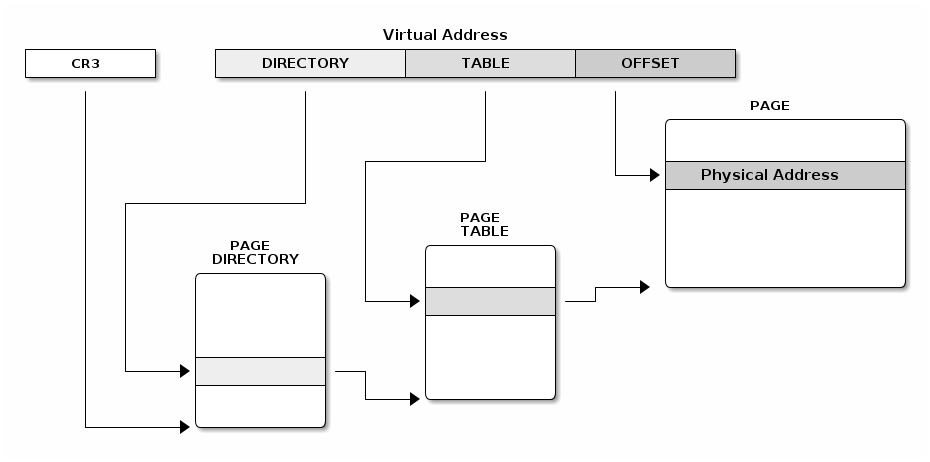
\includegraphics[width=0.95\textwidth]{figures/ch1/linux_va.png}
  \end{center}
  \caption{Formato indirizzo virtuale in Linux}\label{fig:linux_va}
\end{figure}

Quindi per giungere da un indirizzo virtuale ad uno fisico, in Linux si applica il 
\textbf{\textit{page walking}} che consente di prendere l'indirizzo reale in \textbf{\textit{O(1)}}. 
Questo meccanismo viene accelerato in hardware con i TLB che contengono puntatori all'indirizzo 
base della \textbf{\textit{Page Directory}} nel registro \textbf{\textit{CR3}} della CPU.

\subsection{Allocazione delle pagine}
Per decidere quale allocatore utilizzare, Linux introduce il concetto di \textbf{\textit{page order}} 
($0 \leq order \leq 10$). In particolare, quando viene richiesta di un'area di memoria il 
page order indica quante pagine bisogna allocare secondo l'espressione $2^{order}$ (bytes). 
Osservando \cref{fig:order}, la dimensione delle 
pagine cresce all'aumentare dell'ordine.

\begin{figure}[h]
  \begin{center}
    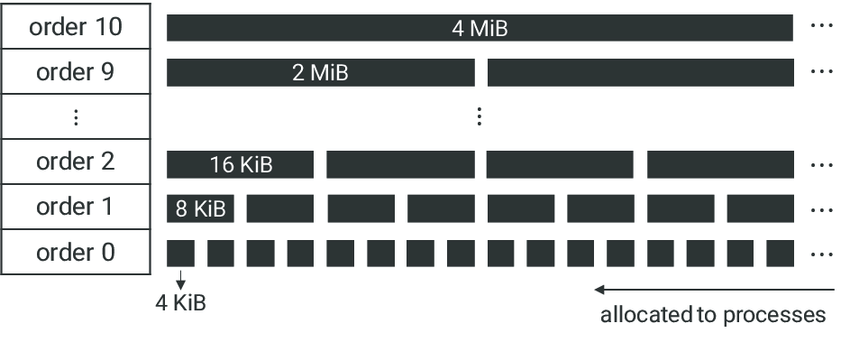
\includegraphics[width=0.95\textwidth]{figures/ch1/Memory-management-in-Linux-via-the-buddy-allocator-algorithm-Memory-spaces-are-divided.png}
  \end{center}
  \caption{Allocazione delle pagine Linux}\label{fig:order}
\end{figure}

Un diagramma di flusso che mostra come vengono gestite le pagine in Linux è mostrato 
in \cref{fig:flowchart-page-allocator} 
(diagramma tratto da \cite{NetfilterTablesVulnerability}).

\begin{figure}[h]
  \begin{center}
    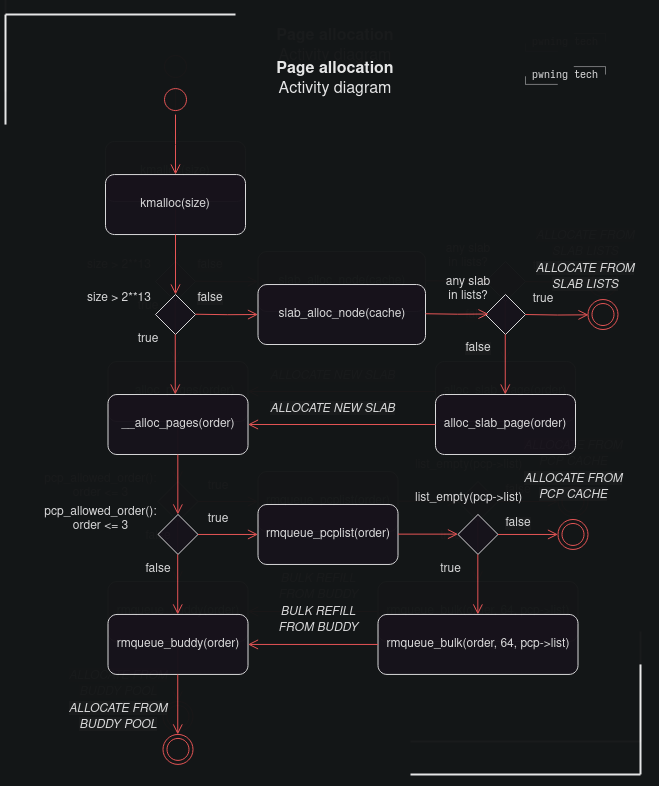
\includegraphics[width=0.7\textwidth]{figures/ch1/activity-diagram-allocator.png}
  \end{center}
  \caption{Diagramma di flusso di come vengono allocate le pagine}\label{fig:flowchart-page-allocator}
\end{figure}


Infatti, la \cref{fig:allocator-per-order}\cite{NetfilterTablesVulnerability}
mostra come il buddy allocator può essere sempre utilizzato, ma utilizza pagine da un pool globale 
condiviso attraverso le CPU (\textit{alloc\_pages()}): il suo intervento causa quindi la 
necessità di bloccare tutte le CPU. Al contrario per piccole allocazioni, fino all'ordine 
$3$, viene utilizzato il \textbf{\textit{per-cpu-page allocator}} (PCP) che mantiene liste 
di piccole pagine nelle cache delle singole CPU e non ha bisogno di un meccanismo di sincronizzazione 
(analogamente al \textit{buddy allocator}). Infine, lo slab allocator si occupa di 
gestire piccole allocazioni nella singola CPU, ma viene invocato dalla funzione 
\textbf{\textit{kmalloc()}}.

\begin{figure}[h]
  \begin{center}
    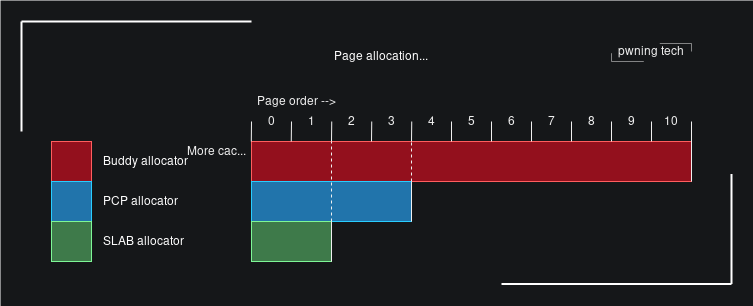
\includegraphics[width=0.95\textwidth]{figures/ch1/allocator-per-order.png}
  \end{center}
  \caption{Allocatore utilizzato in base all'ordine delle pagine}\label{fig:allocator-per-order}
\end{figure}

\paragraph{Anomalie nella gestione delle pagine} L'allocazione delle pagine non avviene 
immediatamente, ma con una modalità \textbf{\textit{just in time}}: ovvero quando una pagina 
virtuale viene acceduta. Ciò avviene in modalità kernel in seguito ad un page fault, durante 
il quale la Page table entry (PTE) viene allocata e aggiornata. Il modello di funzionamento del 
PCP è il seguente: ogni CPU ha una \textbf{\textit{free list}} dalla quale prende le pagine 
quando vengono allocate. La free list viene gestita con delle operazioni \textbf{\textit{drain}} e 
\textbf{\textit{refill}} dalla page list globale (quella utilizzata dal buddy allocator con 
$order \geq 4$). L'attacco in questione mira a far passare il controllo dallo slab allocator
(con il quale vengono allocate le pagine per i \textbf{\textit{sk\_buff (socket buffer)}} al 
buddy allocator forzando un'operazione di drain seguita da una di refill.

\clearpage


\subsubsection{Tecnica \textit{Dirty Pagetable}}

\subsubsection{Superare KASLR}
Per utilizzare la tecnica di privilege escalation presentata in \cref{s:pe-linux}, 
bisogna conoscere l'indirizzo fisico in cui si trova il kernel. Grazie agli script in 
\cite{KernelSig}, è possibile ricavare una signature del kernel con la quale ispezionare 
la memoria. In generale, si tratta di una operazione veloce in quanto il kernel si trova 
allineato ad indirizzi multipli di di $2MiB$ (con la variabile \textbf{\textit{CONFIG\_PHYSICAL\_ALIGN}}). 

Lo script consente di effettuare un attacco bruteforce per individuare l'indirizzo base del 
kernel. In particolare, genera uno snippet di codice $C$ (mostrato di seguito e che può
essere facilmente esteso per supportare diversi kernel). 

\begin{lstlisting}[language=C,style=CStyle,caption="Signature calcolate con lo script fornito dall'autore dell'exploit"]
static int is_kernel_base(unsigned char *addr)
{
	// thanks python
	
	// get-sig kernel_runtime_1
	if (memcmp(addr + 0x0, "\x48\x8d\x25\x51\x3f", 5) == 0 &&
			memcmp(addr + 0x7, "\x48\x8d\x3d\xf2\xff\xff\xff", 7) == 0)
		return 1;

	// get-sig kernel_runtime_2
	if (memcmp(addr + 0x0, "\xfc\x0f\x01\x15", 4) == 0 &&
			memcmp(addr + 0x8, "\xb8\x10\x00\x00\x00\x8e\xd8\x8e\xc0\x8e\xd0\xbf", 12) == 0 &&
			memcmp(addr + 0x18, "\x89\xde\x8b\x0d", 4) == 0 &&
			memcmp(addr + 0x20, "\xc1\xe9\x02\xf3\xa5\xbc", 6) == 0 &&
			memcmp(addr + 0x2a, "\x0f\x20\xe0\x83\xc8\x20\x0f\x22\xe0\xb9\x80\x00\x00\xc0\x0f\x32\x0f\xba\xe8\x08\x0f\x30\xb8\x00", 24) == 0 &&
			memcmp(addr + 0x45, "\x0f\x22\xd8\xb8\x01\x00\x00\x80\x0f\x22\xc0\xea\x57\x00\x00", 15) == 0 &&
			memcmp(addr + 0x55, "\x08\x00\xb9\x01\x01\x00\xc0\xb8", 8) == 0 &&
			memcmp(addr + 0x61, "\x31\xd2\x0f\x30\xe8", 5) == 0 &&
			memcmp(addr + 0x6a, "\x48\xc7\xc6", 3) == 0 &&
			memcmp(addr + 0x71, "\x48\xc7\xc0\x80\x00\x00", 6) == 0 &&
			memcmp(addr + 0x78, "\xff\xe0", 2) == 0)
		return 1;


	return 0;
}

\end{lstlisting}

Una volta trovato l'indirizzo base del kernel, si può aggiungere un offset per trovare 
la variable \textbf{\textit{modprobe\_path}} per effettuare privilege escalation come mostrato 
in \cref{s:pe-linux}.

\subsection{Privilege escalation in Linux}\label{s:pe-linux}
\subsubsection{Sovrascrittura della variabile \textit{modprobe\_path}}
Una tecnica per effettuare privilege escalation in Linux prevede l'utilizzo del programma 
modprobe. Quando viene eseguito un programma in Linux, sostanzialmente viene invocata 
la system-call \textbf{\textit{execve}} a cui sono passati gli argomenti del programma 
e il nome del file stesso. Se il file non è del formato ELF (header non corrisponde a $0x7FELF$) 
invoca modprobe che cercherà di eseguire il programma come modulo. La funzione di seguito 
mostra il codice della funzione \textbf{\textit{call\_modprobe()}} (tratto da \cite{LinuxDocs})

\begin{lstlisting}[language=C,style=CStyle,caption="Invocazione del programma modprobe per la gestione dei programmi dal formato sconosciuto"]
static int call_modprobe(char *module_name, int wait)
{
	struct subprocess_info *info;
	static char *envp[] = {
		"HOME=/",
		"TERM=linux",
		"PATH=/sbin:/usr/sbin:/bin:/usr/bin",
		NULL
	};

	char **argv = kmalloc(sizeof(char *[5]), GFP_KERNEL);
	if (!argv)
		goto out;

	module_name = kstrdup(module_name, GFP_KERNEL);
	if (!module_name)
		goto free_argv;

	argv[0] = modprobe_path;
	argv[1] = "-q";
	argv[2] = "--";
	argv[3] = module_name;	/* check free_modprobe_argv() */
	argv[4] = NULL;

	info = call_usermodehelper_setup(modprobe_path, argv, envp, GFP_KERNEL,
					 NULL, free_modprobe_argv, NULL);
	if (!info)
		goto free_module_name;

	return call_usermodehelper_exec(info, wait | UMH_KILLABLE);

free_module_name:
	kfree(module_name);
free_argv:
	kfree(argv);
out:
	return -ENOMEM;
} 
\end{lstlisting}

L'invocazione del programma modprobe viene fatto leggendo il path da una stringa 
come un array di caratteri nel file \textbf{\textit{kernel/kmod.c}} ed ha come valore di 
default \textbf{\textit{/sbin/modprobe}}. Modificando questa stringa si può eseguire un 
altro programma (malevolo) con i privilegi di amministratore sulla macchina Linux. 

\subsubsection{Superare CONFIG\_STATIC\_USERMODEHELPER}
Nei kernel recenti, questa vulnerabilità è stata mitigata rendendo la variabile \textbf{\textit{modprobe\_path}} 
costante. È possibile superare questo meccanismo di sicurezza utilizzando arbitrary address write 
(AAW) per cercare di sovrascrivere altri file che fanno parte della suite di usermode-helper. 

\subsection{Frammentazione dei pacchetti IP}
Quando un'host invia un pacchetto sulla rete questo non può essere più grande della MTU 
della LAN in cui si trova. La MTU è determinata dal livello data-link e quello IP che 
tipicamente vale $1500$. In \cref{fig:ipv4-header}, è mostrato l'header di un pacchetto IP in cui sono 
evidenziati i campi utilizzati per la frammentazione. 

I campi rilevanti sono:
\begin{itemize}
  \item \textbf{\textit{identification}} ($16$ bit): un numero univoco per la comunicazione in atto (ip sorgente 
    destinazione e campo protocollo). Serve ad identificare univocamente pacchetti frammentati;
  \item \textbf{\textit{flags}} ($3$ bit): flag in cui si indica se sono in arrivo altri frammenti ($MF=1$) oppure 
    se il frammento è l'ultimo ($MF=0$). Inoltre, è possibile chiedere di non frammentare il 
    pacchetto con $DF=1$;
  \item \textbf{\textit{fragment offset}} ($13$ bit): indica da dove partono i dati rispetto 
    al frammento iniziale. Serve per la fase di riassemblaggio;
\end{itemize}

\begin{figure}[h]
  \begin{center}
    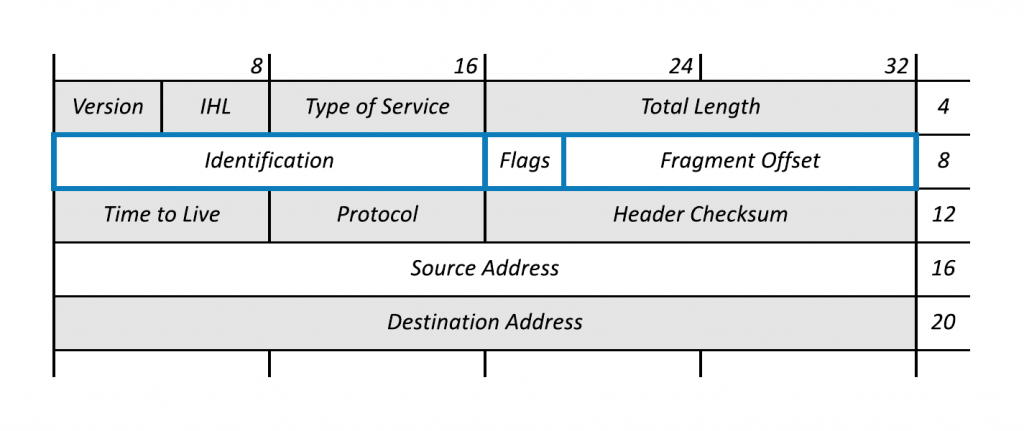
\includegraphics[width=0.95\textwidth]{figures/ch1/IPv4-Headers-Standard-Fragmentation-Highlighted-1024x431.png}
  \end{center}
  \caption{Header di un pacchetto IPv4}\label{fig:ipv4-header}
\end{figure}

\subsubsection{Gestione dei pacchetti frammentati in Linux}
Per i pacchetti IP frammentati, Linux gestisce una struttura dati chiamata \textbf{\textit{IP 
frag queue}} attraverso un albero \textbf{\textit{red-black}} in attesa della ricezione di tutti 
i frammenti (ovvero quando riceve $MF = 0$). Terminati i frammenti, il pacchetto viene 
ricostruito sulla CPU sulla quale è stato processato l'ultimo frammento. Questo comporta 
la migrazione di tutta la free-list con la coda associata su un nuovo processore 
generando un \textbf{\textit{free}} della freelist. 

Ad esempio (\cref{fig:skb-migr}) presa da \cite{NetfilterTablesVulnerability}, se si volesse spostare \textbf{\textit{skb1}} dalla \textbf{\textit{CPU0}} all 
\textbf{\textit{CPU1}}, si può allocare skb1 come frammento di un pacchetto IP e inviare 
\textbf{\textit{skb2}} sulla \textbf{\textit{CPU1}} marcandolo come frammento finale. 
Questo può essere fatto con lo pseudo-codice di seguito:

\begin{lstlisting}[language=C,style=CStyle,caption="Creazione di due frammenti per un pacchetto IP"]
iph1->len = sizeof(struct ip_header)*2 + 64;
iph1->offset = ntohs(0 | IP_MF); // set MORE FRAGMENTS flag 
memset(iph1_body, 'A', 8); 
transmit(iph1, iph1_body, 8); 

iph2->len = sizeof(struct ip_header)*2 + 64; 
iph2->offset = ntohs(8 >> 3); // don't set IP_MF since this is the last packet 
memset(iph2_body, 'A', 56); 
transmit(iph2, iph2_body, 56);
\end{lstlisting}


\begin{figure}[h]
  \begin{center}
    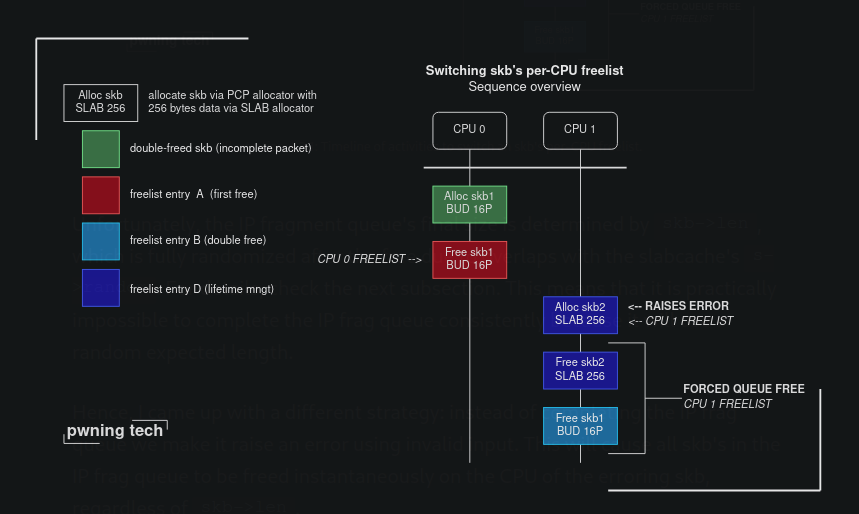
\includegraphics[width=0.95\textwidth]{figures/ch1/switching_skb_cpu-1.png}
  \end{center}
  \caption{Utilizzo della frammentazione IP per spostare un skb da una CPU ad un'altra}\label{fig:skb-migr}
\end{figure}

\subsubsection{Superare CONFIG\_FREELIST\_HARDENED} Nei moderni Kernel, è stato introdotto 
un controllo per assicurare che le freelist del PCP non siano corrotte. Questo meccanismo 
viene aggirato inviando dei pacchetti UDP veri su una socket in ascolto su un indirizzo locale. 
In questo modo, ricevendo i datagrammi UDP si effettuano a ripetizione delle free realizzando 
la \textbf{\textit{spray-free}} dei pacchetti allocati. Infine, si invia un pacchetto frammentato 
che andrà ad impattare le regole nf\_tables configurate all'inizio dell'exploit per attivare 
il primo free.

\begin{lstlisting}[language=C,style=CStyle,caption="Trigger del primo free con un pacchetto frammentato (0x2000)"]
static void privesc_flh_bypass_no_time(int shell_stdin_fd, int shell_stdout_fd)
{
    // ... (skb spray)

    // allocate and free 1 skb from freelist
	df_ip_header.ip_id = 0x1337;
	df_ip_header.ip_len = sizeof(struct ip)*2 + 32768 + 24;
	df_ip_header.ip_off = ntohs((0 >> 3) | 0x2000);  // wait for other fragments. 8 >> 3 to make it wait or so?
	trigger_double_free_hdr(32768 + 8, &df_ip_header);

    // ... (rest of the exploit)
} 
\end{lstlisting}
Un altro problema dei meccanismi di sicurezza di Linux è che quando viene deallocato skb1 
\textbf{\textit{skb1->len}} viene sovrascritto con elementi randomici. L'unico modo per forzare 
il secondo rilascio delle risorse è quello di inviare un pacchetto IP malformato (con body nullo) 
e obbligare il kernel a scartare tutta la \textit{IP frag queue}.

\subsection{Firewall: netfilter API}
Il modulo \textbf{\textit{nf\_tables}} è il backend utilizzato in tutte le distribuzioni 
Linux per \textbf{\textit{iptables}}. Per capire se inoltrare un pacchetto o meno,
netfilter utilizza un algoritmo basato su una macchina a stati configurata con le regole 
degli utenti. Come mostrato in \cref{fig:nf-tables-entity} (tratta da \cite{NetfilterTablesVulnerability}), nftables è organizzato in:
\begin{itemize}
  \item Tables: protocollo da ispezionare
  \item Chains: una catena racchiude un insieme di regole da applicare ad uno specifico insieme di 
    pacchetti;
  \item Rules: regole da applicare ai pacchetti in ingresso alla catena;
  \item Expressions: istruzioni da applicare alla macchina a stati.
\end{itemize}

\begin{figure}[h]
  \begin{center}
    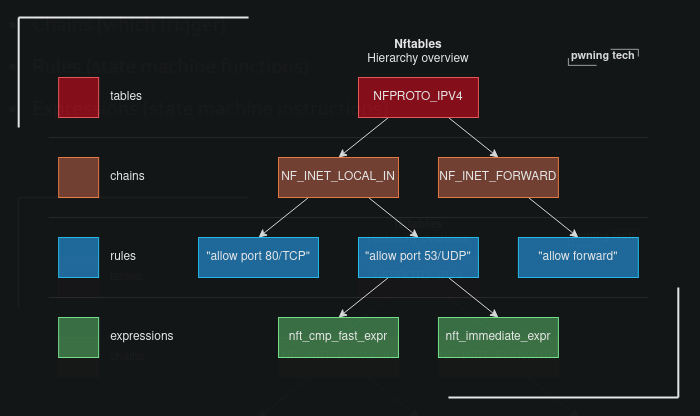
\includegraphics[width=.65\textwidth]{figures/ch1/nf_tables-4.png}
  \end{center}
  \caption{Entità principali di NfTables}\label{fig:nf-tables-entity}
\end{figure}


Un diagramma dinamico del trattamento che può ricevere un pacchetto in netfilter è mostrato 
in \cref{fig:nf_flow}.

\begin{figure}[h]
  \begin{center}
    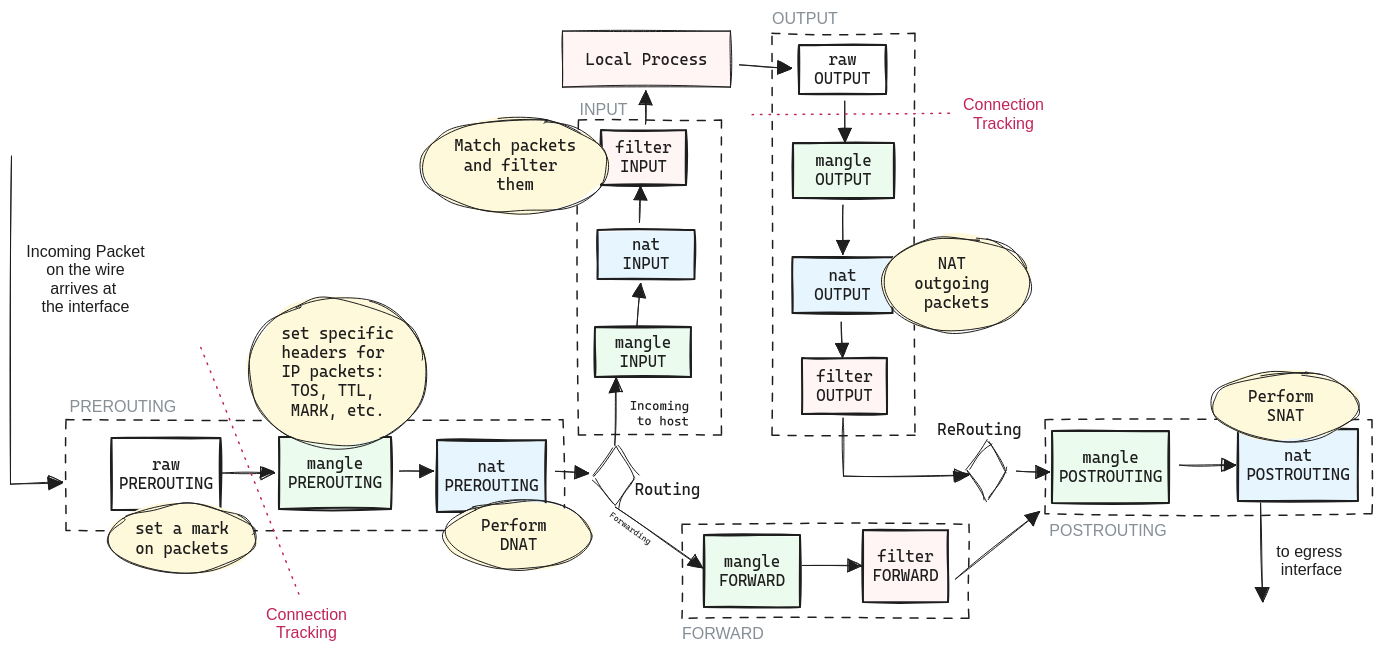
\includegraphics[width=0.95\textwidth]{figures/ch1/Diagrama_linux_netfilter_iptables.png}
  \end{center}
  \caption{Flusso di un pacchetto all'interno di netfilter}\label{fig:nf_flow}
\end{figure}

\subsubsection{Vulnerabilità double free} Essendo molto versatile, \textbf{\textit{nf\_tables}} 
contiene molte vulnerabilità. In questo attacco la vulnerabilità trovata è un double free 
ottenuto forzando netfilter a ri-accettare un pacchetto che era stato marcato come da scartare. 
Ciò avviene a causa del modo con il quale netfilter decide se un pacchetto deve essere scartato o 
meno attraverso un \textbf{verdetto} che deve essere assegnato da una funzione \textbf{hook}. 
Di seguito, è riportata la funzione che genera la vulnerabilità. In particolare, la funzione 
effettua un ciclo su tutte le regole registrate e controlla cosa fare con il pacchetto (
accettare o scartare). Nel caso di \textbf{\textit{NF\_DROP}}, la funzione costruisce un 
valore di ritorno con la macro \textbf{\textit{NF\_DROP\_GETERR()}} a cui è possibile far 
tornare \textbf{\textit{NF\_ACCEPT}}. Quindi, quando si entra nel branch \textbf{\textit{NF\_DROP}}
si effettua il primo \textbf{\textit{free}} del double free; mentre ritornando \textbf{\textit{NF\_ACCEPT}}
ci si predispone per la seconda deallocazione che sarà effettuata quando il pacchetto non 
sarà più utile.

\begin{lstlisting}[language=C,style=CStyle,caption="Funzione nf_hook_slow che genera la vulnerabilit"]
// looping over existing rules when skb triggers chain
int nf_hook_slow(struct sk_buff *skb, struct nf_hook_state *state,
         const struct nf_hook_entries *e, unsigned int s)
{
    unsigned int verdict;
    int ret;

    for (; s < e->num_hook_entries; s++) {
        // malicious rule: verdict = 0xffff0000
        verdict = nf_hook_entry_hookfn(&e->hooks[s], skb, state);  

        // 0xffff0000 & NF_VERDICT_MASK == 0x0 (NF_DROP)
        switch (verdict & NF_VERDICT_MASK) {  
        case NF_ACCEPT:
            break;
        case NF_DROP:
            // first free of double-free
            kfree_skb_reason(skb,
                     SKB_DROP_REASON_NETFILTER_DROP);  
            
            // NF_DROP_GETERR(0xffff0000) == 1 (NF_ACCEPT)
            ret = NF_DROP_GETERR(verdict);  
            if (ret == 0)
                ret = -EPERM;
            
            // return NF_ACCEPT (continue packet handling)
            return ret;  

        // [snip] alternative verdict cases
        default:
            WARN_ON_ONCE(1);
            return 0;
        }
    }

    return 1;
}
\end{lstlisting}

Ciò è possibile a causa del modo con il quale viene generato il verdetto. Infatti, i 16 bit 
più significativi dovrebbero essere negativi, ma la funzione non verifica questa condizione 
e quindi rende possibile ritornare un valore positivo che viene tradotto in 
\textbf{\textit{NF\_ACCEPT}}\cite{Patch}.

\subsection{Linux user namespaces} 
L'attacco utilizza l'isolamento a livello di processo offerto da Linux. In particolare, 
per agire indisturbati sulle tabelle netfilter viene creato un namespace attraverso la 
systemcall unshare. Di fatto, l'exploit viene eseguito in un container rudimentale 
e ha bisogno della variabile \textbf{\textit{sysctl kernel.unprivileged\_userns\_clone
kernel.unprivileged\_userns\_clone = 1}} (disponibile default in tutte le maggiori 
distribuzioni Linux). 

\begin{lstlisting}[language=C,style=CStyle,caption="Setup network namespace come utente non privilegiato"]
static void do_unshare()
{
    int retv;

    printf("[*] creating user namespace (CLONE_NEWUSER)...\n");
    
	// do unshare seperately to make debugging easier
    retv = unshare(CLONE_NEWUSER);
	if (retv == -1) {
        perror("unshare(CLONE_NEWUSER)");
        exit(EXIT_FAILURE);
    }

    printf("[*] creating network namespace (CLONE_NEWNET)...\n");

    retv = unshare(CLONE_NEWNET);
    if (retv == -1)
	{
		perror("unshare(CLONE_NEWNET)");
		exit(EXIT_FAILURE);
	}
}
\end{lstlisting}

\clearpage
\section{Attacco}
Come illustrato in \cref{s:basics}, l'attacco prevede tre 
passi fondamentali:
\begin{itemize}
  \item setup del namespace e delle tabelle netfilter;
  \item trigger del double free con pacchetti IP frammentati;
  \item sovrascrittura delle pagine;
\end{itemize}
Un PoC che sfrutta la vulnerabilità è presente in \cite{ExploitPoC}.
\subsection{Preparazione del kernel}

\subsection{Configurazione kernel: socket Netlink}

\subsection{Exploit della vulnerabilità}

\clearpage

\section{Mitigazione della vulnerabilità}
La funzione \textbf{\textit{nf\_hook\_slow()}} è stata patchata. In particolare, è stata 
eliminata la macro \textbf{\textit{NF\_DROP\_GETERR}} poichè NF\_QUEUE non è utilizzato da 
nftables.\cite{Patch}.

\begin{lstlisting}[language=C,style=CStyle,caption="Commit applicato per mitigare la vulnerabilità"]
--- a/net/netfilter/nf_tables_api.c
+++ b/net/netfilter/nf_tables_api.c
@@ -10988,16 +10988,10 @@ static int nft_verdict_init(const struct nft_ctx *ctx, struct nft_data *data,
 	data->verdict.code = ntohl(nla_get_be32(tb[NFTA_VERDICT_CODE]));
 
 	switch (data->verdict.code) {
-	default:
-		switch (data->verdict.code & NF_VERDICT_MASK) {
-		case NF_ACCEPT:
-		case NF_DROP:
-		case NF_QUEUE:
-			break;
-		default:
-			return -EINVAL;
-		}
-		fallthrough;
+	case NF_ACCEPT:
+	case NF_DROP:
+	case NF_QUEUE:
+		break;
 	case NFT_CONTINUE:
 	case NFT_BREAK:
 	case NFT_RETURN:
@@ -11032,6 +11026,8 @@ static int nft_verdict_init(const struct nft_ctx *ctx, struct nft_data *data,
 
 		data->verdict.chain = chain;
 		break;
+	default:
+		return -EINVAL;
 	}
 
 	desc->len = sizeof(data->verdict);
--  
\end{lstlisting}
\clearpage

\nocite{*}

\bibliography{refs.bib}
\end{document}
